
The data presented were taken in $2015$ using $\Datura$, a $\eudet$-type beam telescopes, which was operated with EUDAQ, cf.~section~3 and~4. 
The results presented in this section have been obtained using the EUTelescope software described in section~\ref{sec:offline}.
The set-up does not include any additional DUT, only six $\Mimosa$ telescope planes. 
Track fits are performed using the GBL formalism and track residuals, i.e.\ the distance between the track fit and the measured hit,
 are calculated for each telescope plane. 
 

\subsection{Data analysis flow}
\label{sec:datura-nodut}

After conversion from raw $\Mimosa$ data, a hot pixel search is performed marking pixels with firing frequencies above a certain threshold.
Clusters are formed from fired, adjacent pixels and translated from two-dimensional entities on the individual telescope planes into hits in a global three-dimensional reference frame.
Clusters containing at least one hot pixel are removed from the analysis. 
Track triplets are built from hits in the three upstream and three downstream planes separately: 
First, doublets are defined by straight lines from all hits in plane\,0 to all hits in plane\,2. 
A valid triplet is found, if a matching hit in plane\,1 is present, non-valid triplets are discarded.  
Triplet isolation is ensured by rejecting all triplets whose extrapolation at a chosen $z$-coordinate approaches other triplet extrapolations closer than $\unit{300}{\upmu\meter}$,
 the $z$-coordinate being the centre between plane\,2 and plane\,3. 
The procedure is repeated for the downstream planes. 
Matching triplets from the up- and downstream planes are identified by isolated triplets that intersect within a radius of $\unit{100}{\upmu\meter}$, again at the centre between plane\,2 and plane\,3. 
In turn, GBL tracks are formed by the six hits belonging to the matched triplets. 
For offline alignment, the GBL tracks are passed to Millepede-II in order to determine shift and rotation alignment constants for every telescope plane.
After applying the alignment corrections, the above track finding is repeated, and the final GBL tracks are calculated. 
These tracks can be formed in a \textrm{biased} or in an \textrm{unbiased} way, where biased tracks include the measured hit information of every plane in contrast to unbiased tracks,
 that omit the hit information of the plane under investigation. 

\subsection{Multiple scattering and residuals}
\label{sec:resmultiple}

The figure of merit for a beam telescope is its track resolution\footnote{also called pointing resolution} $\sigmatb$ ($\sigmatu$).
It defines the precision with which a particle trajectory can be determined for an biased (unbiased) track. 
This quantity is a function of the track path, i.e.\ it is not constant along the trajectory. 
%The timing resolution is largely dependent on the readout speed of the used sensors, their buffer sizes and the data acquisition system. 
It depends on the intrinsic resolution $\sigmai$ of the sensors, that have been used to measure the hits belonging to the track, the number of measurements and their positions
 as well as the multiple scattering of the beam particles.
Various methods exist to perform the calculation of the track resolution. 
In the formalism of GBL, the track resolution results from a single, global $\chi^2$-fit of a track model to all measured hits including their measurement uncertainties (intrinsic resolution)
 and scattering angle uncertainties along the trajectory. 
% 
%The resolution of a telescope $\sigma_{\textrm{Tel}}$ can be expressed by
%
%\begin{equation}
%\label{eq:telescopepointing}
%\sigma_{\textrm{Tel}}^2 = k \cdot \sigmai^2
%\end{equation}
%
%\noindent
% with the geometric scaling factor $k$ in turn written as
%
%\begin{equation}
% k = \frac{\sum_i^N z_i^2}{N \cdot \sum_i^N z_i^2 - \left( \sum_i^N z_i \right)^2} \,,
%\end{equation}
%
%\noindent
% assuming all $N$ telescope planes have the same intrinsic resolution $\sigmai$. 
%The distance of the $i$-th telescope plane to the DUT positioned at $z=0$ is then $z_i$ .
%For a symmetric set-up with the DUT at the centre of the telescope and the up- and downstream planes equally spaced, $k$ reduces to $k = 1/N$. 
%
Multiple Coulomb scattering causes angular deflection of charged particles traversing any medium.
The angular scattering distribution is centred around zero
 and the width depends on the particle energy, particle type and the radiation length of the matter traversed~\cite{ref:scatteringhighland}.
An approximation for high energy protons, that is accurate to 11\,\% for all atomic numbers $Z$, yields a closed form for the distribution width in the transverse plane~\cite{ref:PDG-2014}

\begin{equation}
\label{eq:multiplescattering}
\Theta_{0} = \frac{13.6\,\mega\electronvolt}{\beta c p} \cdot z
\sqrt{\varepsilon}
\cdot \left( 1 + 0.038 \ln{\left( \varepsilon \right) } \right) \,,
\end{equation}

\noindent with the velocity $\beta c$, the momentum $p$ and the charge number $z$ of the traversing particle. 
The expression $\epsilon = x \per X_0$ is the material budget, as defined in section~\ref{sec:sensors}.
%
Equation~(\ref{eq:multiplescattering}) demonstrates the advantage of using thin sensors, since the angular deflection due to multiple scattering increases with the material budget.
This is especially important at low-energy beams, such as the DESY-II test beam, as the distortion increases towards lower energies.
As the beam particles interact with both the sensors and the air, contributions to the amount of multiple scattering from either source have to be considered.
At high-energy hadron beams, the contribution from multiple scattering can in general be neglected. 
 
The biased (unbiased) residual defined as a quantity per track is the distance between the measured hit and the biased (unbiased) track fit. 
With a known or estimated biased track resolution, i.e.\ all $\sigmai(z_i)$ are known or estimates exist,
 the width of the distribution of the biased residuals for a set of tracks can be expressed for all positions $z = z_i$ as

\begin{equation}
 \label{eq:telescoperesolutionequation1}
 \rbiased^2(z) = \sigmai^2(z) - \sigmatb^2(z).
\end{equation}

\noindent
The biased residuals at a considered plane $i$ are always smaller for the wide configuration in comparison to the narrow one and decrease towards lower beam energies. 
These effects stem from the term $\sigmatb$: 
Qualitatively, the biased track resolution increases with larger lever arms $\dz$, as an uncertainty in the deflection angle is boosted with larger distance,
 and converges towards the intrinsic resolution in the limit of large deflection. 
Hence, the difference between $\sigmai$ and $\sigmatb$ decreases. 

If the hit measurement of a DUT at $\zdut$ or of a telescope plane at position $z_i$ is not included in the fit,
 the width of the distribution of the unbiased residuals at these positions reads~\cite{ref:eudetreport200902}
 
\begin{equation}
\runbiased^2(z) = \sigmai^2(z) + \sigmatu^2(z).
\label{eq:telescoperesolutionequation2} 
\end{equation}

\noindent
Both the biased and the unbiased residual distributions are a function of the track resolution and therefore exhibit the same dependencies.
It should be noted that the unbiased track resolution at a sensor plane can be larger than the intrinsic resolution. 
On the contrary, the biased track resolution is always smaller than or equal to the intrinsic resolution of the sensor planes. 

The biased pull of a track is defined as the ratio of the biased residual over the predicted biased residual width

\begin{equation}
 \textrm{pull}_{\textrm{b}} \equiv \pb = \frac{\rbiased}{\sqrt{\sigmai^2 - \sigmatb^2}}.
 \label{eq:pull}
\end{equation}

\noindent
The biased pull distributions are normally distributed and centred at zero with a width of one, $N(0,1)$, if the material and the scattering therein is known and correctly described. 
A width larger than one originates from an underestimated residual prediction $\sqrt{\sigmai^2 - \sigmatb^2}$, which in turn stems from either an underestimated intrinsic resolution
 or an overestimated track resolution. 
The latter is caused by either an overestimated material budget or overestimated deflection angles. 

\begin{table}[tbp]
 \begin{center}
  \begin{tabular}{r|r|r|c|c|c|c||c}
  \multicolumn{3}{c|}{} & \multicolumn{5}{c}{$\sigma_{\sigmai}$ in \%}\\
  \multicolumn{3}{c|}{} & \multicolumn{3}{c|}{per plane} & all planes& $\sqrt{\sum x_i^2}$\\
  \multicolumn{3}{c|}{} &$E\pm5\,\%$ & $\Theta\pm1\,\%$ & fit range & rms &  \\ \hline
  6\,GeV & 20 mm   &  biased  &   &  &  &  &    \\
         & ×       & unbiased &   &  &  &  &    \\
	 & 150 mm  &  biased  &   &  &  &  &    \\
	 & ×       & unbiased &   &  &  &  &    \\ \hline
  2\,GeV & 20 mm   &  biased  &   &  &  &  &    \\
         & ×       & unbiased &   &  &  &  &    \\
	 & 150 mm  &  biased  &   &  &  &  &    \\
	 & ×       & unbiased &   &  &  &  &    \\ 
  %× & × & × & ×
  \end{tabular}
    \caption[Systematic uncertainties for plane\,0]{Systematic uncertainties in determination of the intrinsic resolution for plane\,0, listed for biased and unbiased track fits and the two geometries.
  For unbiased tracks in the wide geometry, the uncertainty of the intrinsic resolution could not be calculated as the measured residual is smaller than the calculated track resolution.}
  \label{tab:uncerts}
 \end{center}
\end{table}

A critical aspect of this analysis is the choice between biased and unbiased residuals. 
In principal, both choices lead to compatible results if the material in the beam and the deflection due to multiple scattering therein is correctly described. 
%With biased residuals, only one fit has to be performed, whereas for unbiased residuals, a new fit has to be formed for every plane under investigation. 
Systematic uncertainties effect the track resolution, the predicted residual width, and finally the derived intrinsic resolution. 
The impact of systematic uncertainties on the result, however, differs between the biased and the unbiased methodology as more information is used in the biased track fits. 
If the pulls distribution resembles $N(0,1)$, equations~(\ref{eq:telescoperesolutionequation1}) and~(\ref{eq:telescoperesolutionequation2}) hold and the systematic uncertainties of the intrinsic resolution
 are estimated based on uncertain beam energy and uncertain deflection angle using the GBL formalism. 
%Firstly, the residuals have been obtained from data assuming an intrinsic resolution of $\sigmai = \unit{3.3}{\micro\meter}$ and secondly the track resolution is calculated. 
%Finally, the intrinsic resolution is calculated as $\sigmai = \sqrt{\rbiased^2 + \sigmatb^2}$ or $\sigmai = \sqrt{\runbiased^2 - \sigmatu^2}$ for biased and unbiased track fits, respectively. 
The beam energy is varied by 5\,\%. 
The original systematic uncertainty of the scattering distribution width $\Theta_{0}$ of $11\,\%$ is experimentally constrained to 1\,\%, as is shown in section~\ref{sec:measurements}. 
All systematic uncertainty contributions for the two set-ups are listed in table~\ref{tab:uncerts} as per plane and the RMS over all planes. 
It shows, that the choice of biased track fits results in smaller systematic uncertainties compared to unbiased track fits. 
Additionally, there is a systematic uncertainty of the method itself, as it predicts slightly different intrinsic resolutions for each plane, which changes between geometries,
 i.e.\ it is not dominantly caused by an actual difference in intrinsic resolution. 
The spread in intrinsic resolution over all planes is 1\,\% and 2\,\% for the wide and the narrow geometry, respectively, for both biased and unbiased track fits. 

The rather large uncertainty of the scattering distribution width given in equation~(\ref{eq:multiplescattering}) and hence significant impact on the final results can be diminished: 
In case the formula's estimate differs from the actual straggling of beam particles in the given material, the predicted track resolution is systematically affected, and therefore the pull distribution. 
Hence, the estimator $\sigmahat$ does not converge towards the true $\sigmai$. 
Since the intrinsic resolution is independent of the plane spacing $\dz$, a comparison at two precisely measured spacings allows for a calibration of $\Theta_0$ at a given beam energy. 
Thereto, a global energy dependent factor $\kappa$ is introduced that is constant as a function of sensor threshold and geometry

\begin{equation}
 \Theta_{\textrm{corr}} = \kappa(E) \cdot \Theta_0.
 \label{eq:thetacorr}
\end{equation}

\noindent
The value $\kappa$ is determined iteratively under the constraint that the resulting intrinsic resolution for the two geometries agree within 10\,nm.
The uncertainty of $\kappa$ is defined as the range for which the intrinsic resolution of the wide geometry equals the central value plus/minus one standard deviation of the narrow geometry. 
If $\kappa$ differs significantly from one and/or depends on the beam energy is to be determined with data in section~\ref{sec:measurements}. 


\subsection{Performance measurements with DATURA}
\label{sec:measurements}

Measurements of particle trajectories were performed to verify the performance of the $\Datura$ telescope at various beam energies, sensor thresholds, and sensor spacings. %~\cite{ref:thomas}.
The biased residual and biased pull distributions have been obtained for every sensor plane as described in sections~\ref{sec:datura-nodut} and~\ref{sec:resmultiple}. 
% By considering one telescope plane as a DUT, equation~(\ref{eq:telescoperesolutionequation}) is modified under the assumption that $\sigmai = \sigma_{\textrm{DUT}} = \sigma_{\textrm{M26}}$,
%  leading to
% 
% \begin{equation}
% \label{eq:telescoperesolutionequation_2}
% \sigmameas^2 = \sigma_{\textrm{M26}}^2 \cdot \left( 1 + k_5 \right) +
% \sigma_{\textrm{MS}}^2\,,
% \end{equation}
Since the intrinsic resolution is not a priori known, an initial estimate of the intrinsic resolution $\sigmahat$ is used as an input to the GBL track fitting. 
The width of the pull distributions is iteratively used to update the estimate $\sigmahat$.
This procedure converges towards the true intrinsic resolution within the uncertainties and yields compatible results for the two different geometries for an appropriate choice of $\kappa$. 
It should be noted that an initial estimate close to the converged value does not yield smaller uncertainties on the converged value compared to a bad initial estimate.
%The systematic uncertainty of the converged estimate is independent of the iteration process.
%A mismatch in intrinsic resolution for the two cases is corrected by varying $\kappa$, cf.~equation~(\ref{eq:thetacorr}) and repeating the iterative method until the intrinsic resolutions equal


\begin{figure}[tbp]
  \centering
  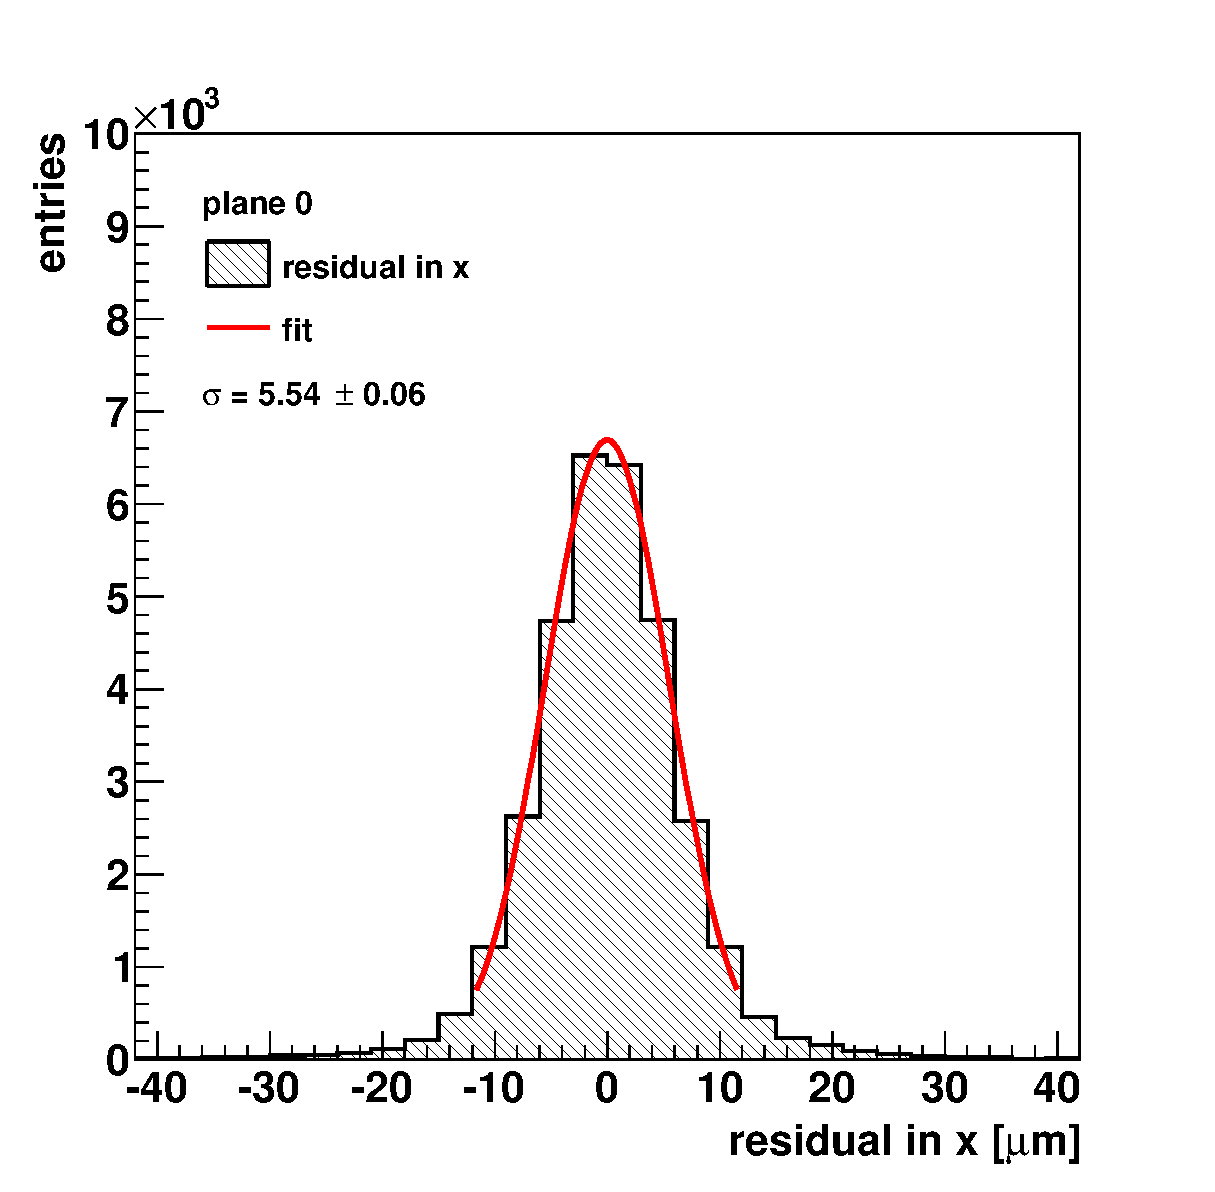
\includegraphics[width=0.49\textwidth]{figures/0x} \put(-50,155){(A)}
  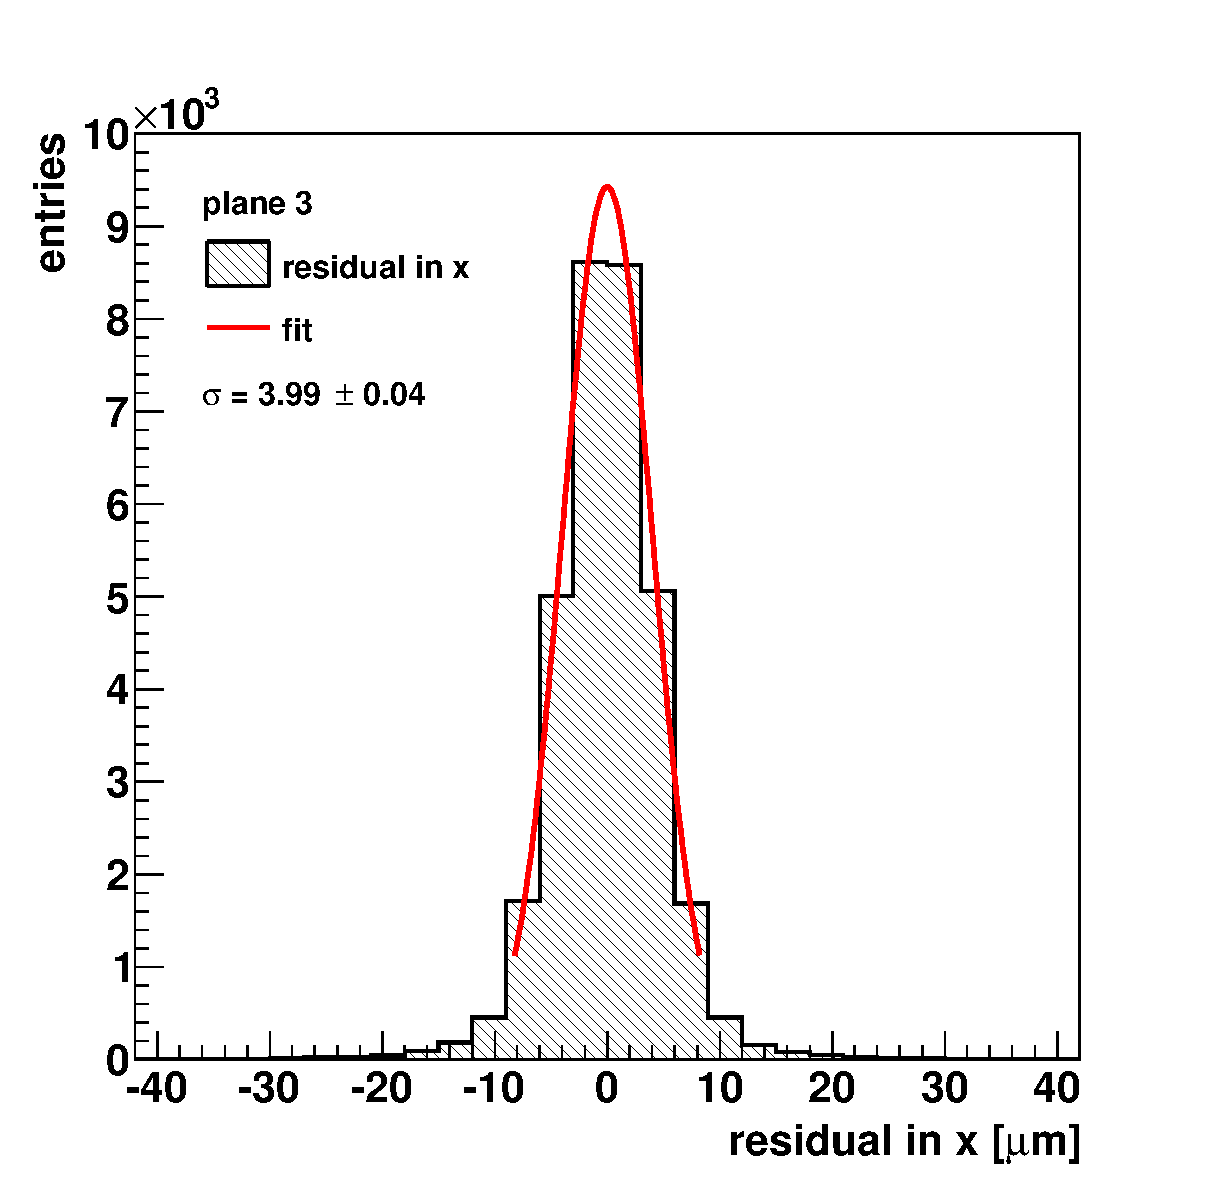
\includegraphics[width=0.49\textwidth]{figures/3x} \put(-50,155){(B)}\\
  %\includegraphics[width=0.45\textwidth]{figures/resis_upstream/1x.pdf}
  %\includegraphics[width=0.45\textwidth]{figures/resis_upstream/1y.pdf}
  %\includegraphics[width=0.45\textwidth]{figures/resis_upstream/2x.pdf}
  %\includegraphics[width=0.45\textwidth]{figures/resis_upstream/2y.pdf}
  %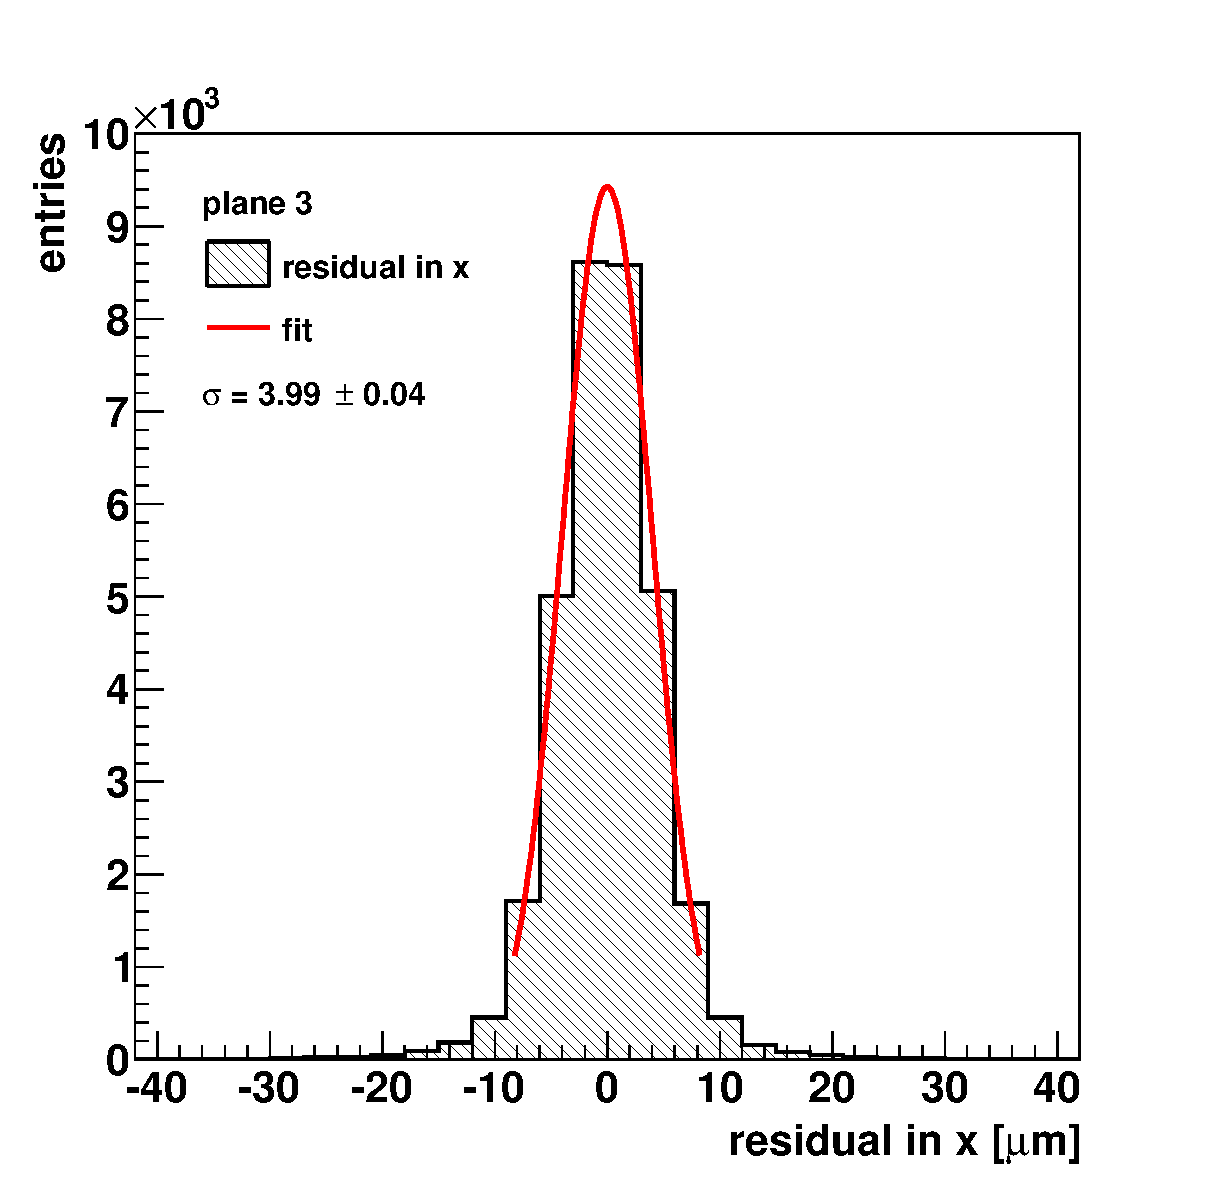
\includegraphics[width=0.49\textwidth]{figures/3x} \put(-50,155){(C)}
  %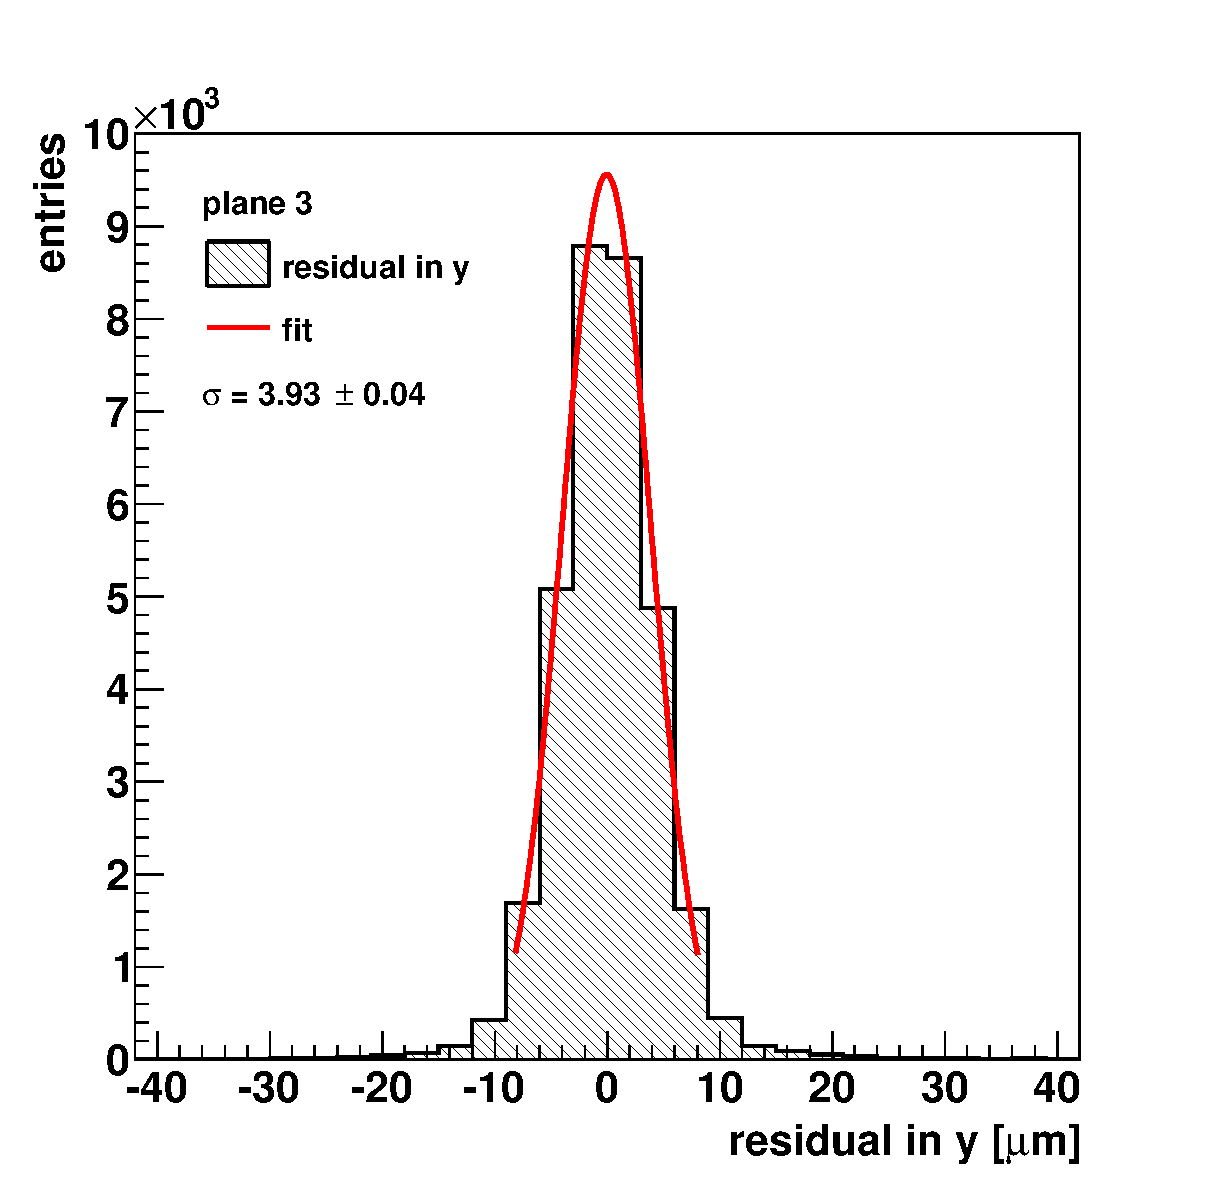
\includegraphics[width=0.49\textwidth]{figures/3y} \put(-50,155){(D)}
  %\includegraphics[width=0.45\textwidth]{figures/resis_downstream/4x.pdf}
  %\includegraphics[width=0.45\textwidth]{figures/resis_downstream/4y.pdf}
  %\includegraphics[width=0.45\textwidth]{figures/resis_downstream/5x.pdf}
  %\includegraphics[width=0.45\textwidth]{figures/resis_downstream/5y.pdf}
  \caption[Residual examples to determine the $\Datura$ telescope's resolution]{
  Biased residual distributions measured with the $\Datura$ telescope at 6\,GeV with a plane spacing of $\dz = 20\,\milli\meter$. 
  The measured residuals in the $x$-direction for plane $0$ (A) and plane $3$ (B) are shown.}
  \label{fig:residualexample1}
\end{figure}

\noindent
%with $k_5$ being the geometric scaling factor for a telescope consisting of five planes. 
%The value of $k_5$ depends on the geometry itself and on which telescope plane is considered as DUT. 
%This configuration with five planes used as beam telescope and one plane as DUT is referred to as \textit{gauge configuration}. 

Figure~\ref{fig:residualexample1} shows an example of biased residual distributions in $x$ for a telescope sensor spacing of $\dz = 20\,\milli\meter$,
 a beam energy of 6\,GeV, and a sensor threshold setting of $\noise = 6$. 
According results for the $y$-direction, further planes and the wide geometry are omitted. 
The distributions are fitted with a Gaussian, from which the residual width $\rbiased$ is determined. 
For plane\,3, the biased residual width in the $x$-direction is 

\begin{equation}
\left( 2.88\,\pm\, 0.009\,\textrm{(stat.)}\,\pm\, 0.06\, \textrm{(sys.)}\right)\,\micro\meter. 
\end{equation}

\noindent
As the systematic uncertainty is the dominant uncertainty, the statistical one is not neglected for the further analysis. 
It should be noted that the residuals feature non-Gaussian tails, as is expected from the underlying physics of the scattering mechanism~\cite{ref:PDG-2014}. 
The measured residual width used in this work is defined as the width of a Gaussian fit on the centre $95.5\,\%$ (2.0 standard deviations) of the residual distribution.
The biased residual width for the outer plane\,0 is smaller than the width obtained from plane\,3.
This is expected due to the fact that the track extrapolation to the inner sensors is performed from both sides, and hence is comparatively more precise than for the outer sensors,
 where the extrapolation can only be performed from one direction. 
Therefore, in equation~(\ref{eq:telescoperesolutionequation1}) the difference between $\sigmai$ and $\sigmatb$ decreases from the centre sensor planes to the outer ones. 

% \begin{figure}[hbtp]
% \centering
% 
% \caption[Residual examples to determine the DATURA telescope's
% resolution. Downstream lever arm]{Residual examples to determine the DATURA
% telescope's resolution from the downstream lever arm. From top to bottom: The
% measured residuals for planes $3$, $4$ and $5$, left for $X$ direction, right
% for $Y$ direction. Each sensor plane was considered as a passive layer during
% the track reconstruction.}
% \label{fig:residualexample2}
% \end{figure}

\begin{figure}[btp]
  \centering
  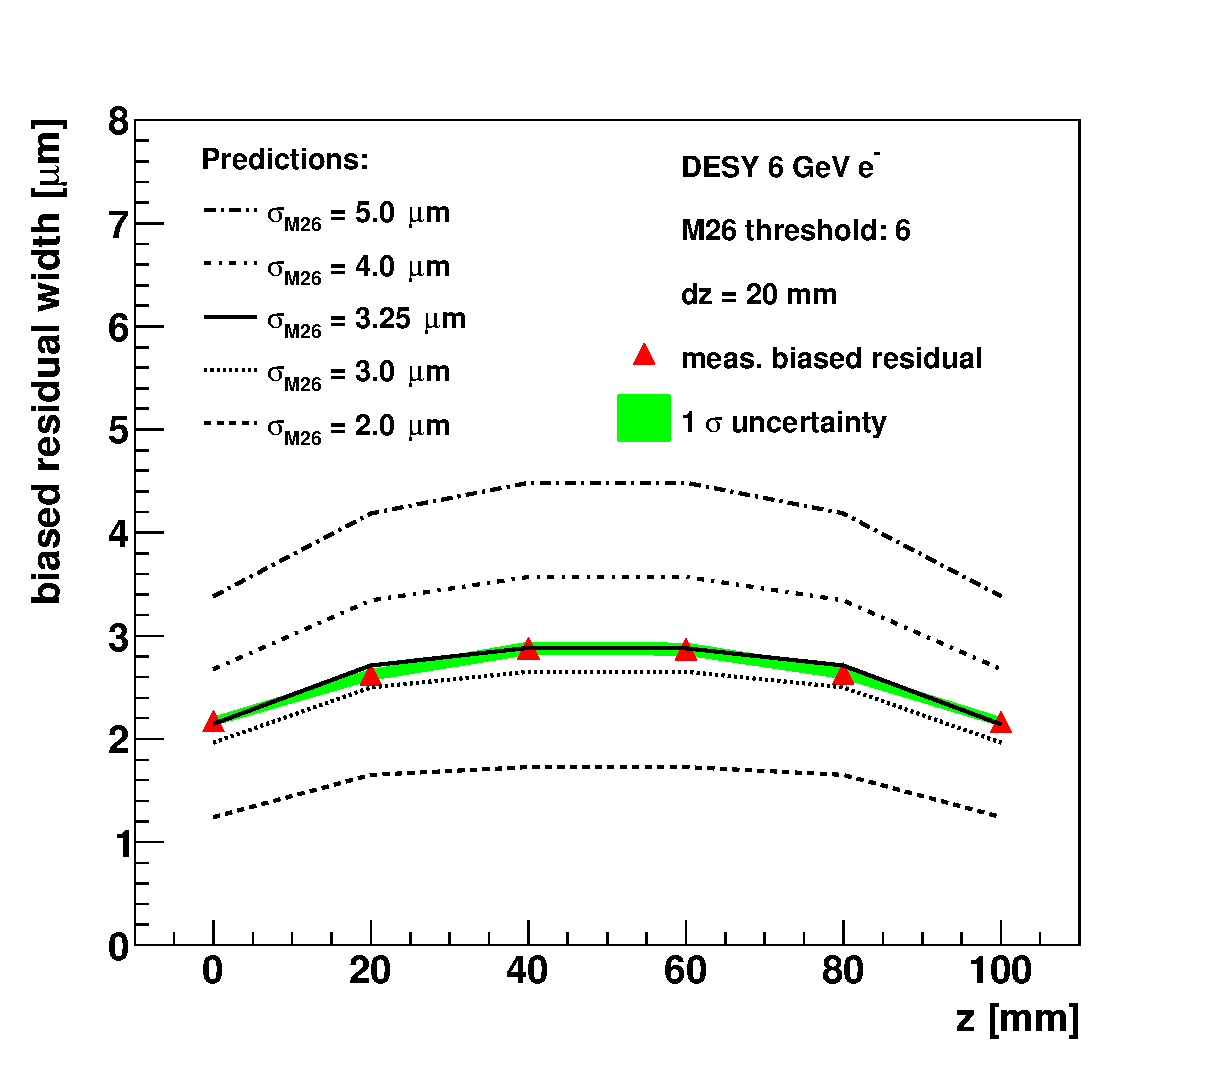
\includegraphics[width=0.49\textwidth]{figures/res_vs_z_20}  \put(-36,160){(A)} % was thin_smiley.pdf
  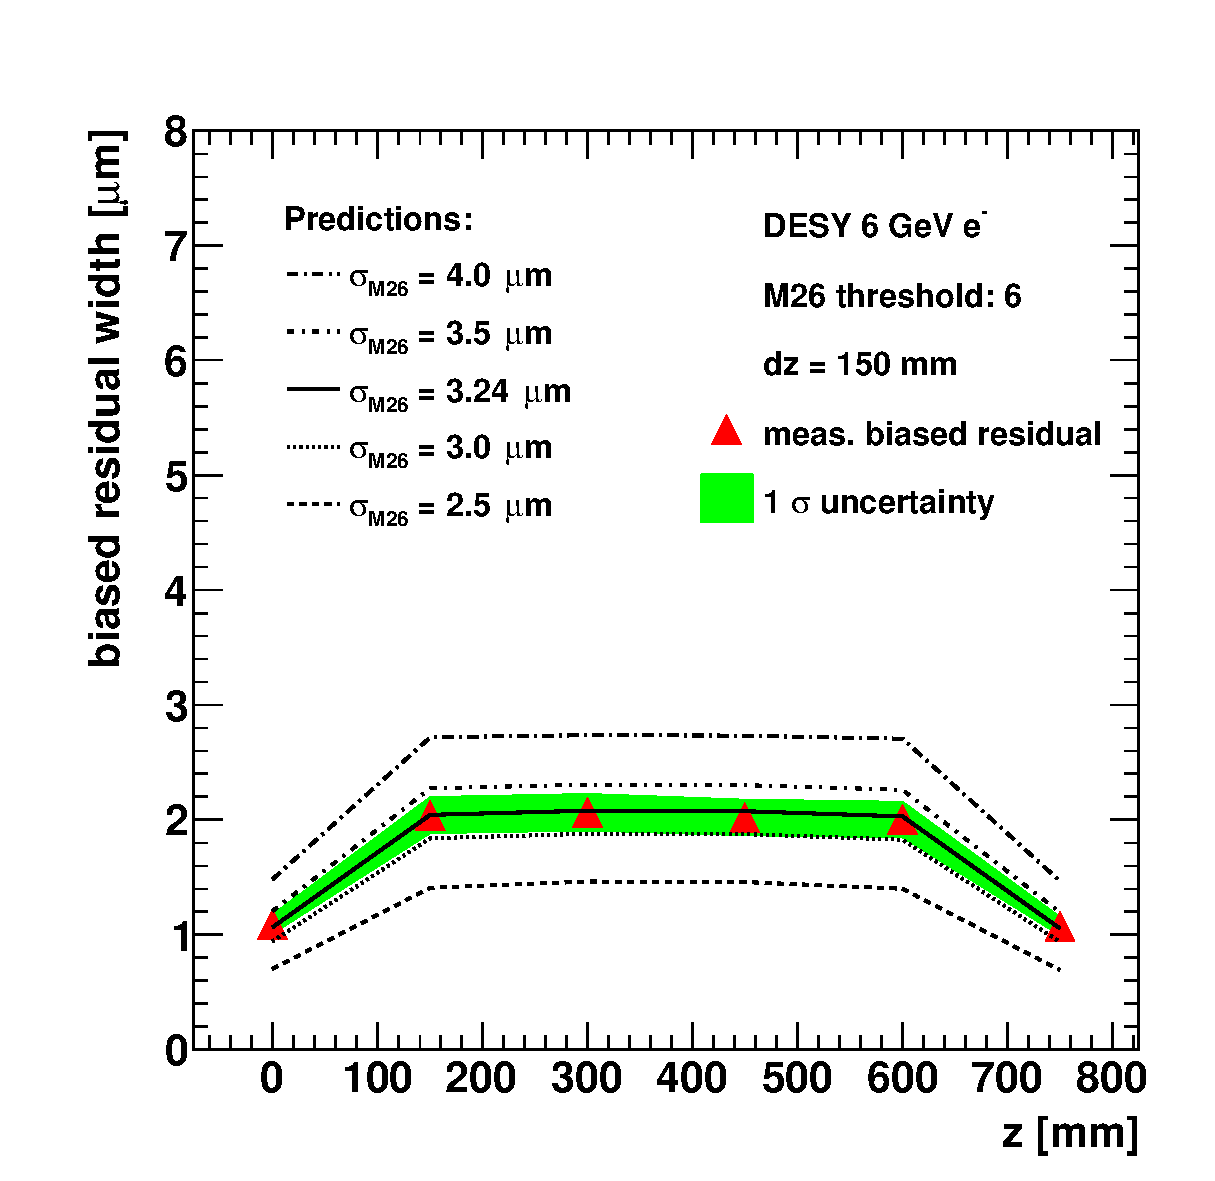
\includegraphics[width=0.49\textwidth]{figures/res_vs_z_150} \put(-36,160){(B)} % was wide_smiley.pdf
  %\caption[Intrinsic telescope sensor resolution at $20\,\milli\meter$ and $150\,\milli\meter$ plane spacing~\cite{ref:thomas}]{Intrinsic telescope sensor resolution at $20\,\milli\meter$ (top)
  % and $150\,\milli\meter$ (bottom) plane spacing.
  \caption[The measured residual widths of each telescope plane.]{
  The measured residual widths of each telescope plane are shown in both the $x$- and $y$-direction for a plane spacing of $\dz = 20\,\milli\meter$ (A) and $\dz = 150\,\milli\meter$ (B).
  The black line shows the predicted residual width at $\sigmam = 3.25\,\upmu\meter$, the green band the measurement standard deviation.
  %Dotted and dashed lines indicate the predicted residual widths, in case differing intrinsic resolutions are assumed.
  %Data was taken at a sensor threshold of $\noise = 6$ and using 6\,GeV electrons at DESY-II.
  }
  \label{fig:smiley}
\end{figure}


The six measured residual widths in the $x$-direction at a beam energy of 6\,GeV and a sensor threshold $\noise = 6$ for both the narrow plane spacing of $\dz = 20\,\milli\meter$
 and the wide spacing of $\dz = 150\,\milli\meter$ are shown in figure~\ref{fig:smiley} (A) and (B), respectively. 
As expected, the residuals at a considered plane $i$ are always smaller for the wide configuration in comparison to the narrow one, cf.~section~\ref{sec:resmultiple}.
%Also, the residuals decrease towards lower beam energies. 
%These effects stem from the term $\sigmatb$ in equation~(\ref{eq:telescoperesolutionequation1}): 
%(1) Qualitatively, the spatial uncertainty of the extrapolation to the next plane increases with larger lever arms $\dz$. 
%(2) The biased track resolution tends towards the intrinsic resolution for increased scattering. 
%Hence, the difference between $\sigmai$ and $\sigmatb$ decreases. 

%The energy dependent width of the scattering angle distribution increase the uncertainty with decreasing energy, c.f.\.equation~\ref{eq:multiplescattering}. 
%In the former term, the geometric scaling factor is larger in the wide configuration, in the latter $\sigma_{\textrm{MS}}$ increases with decreasing beam energy. 

%In order to find the best estimate of the intrinsic sensor resolution, a $\chi^2$ minimisation is performed. 
%Inputs to this minimisation are the twelve measured residuals widths $\sigmameas$ at a sensor threshold of $\noise = 6$ and a beam energy of 6\,GeV. 
%These are compared to analytical estimates of the residuals $\sigmahat$, which depend on the known geometry of the set-up, its material budget, the beam energy,
% and the intrinsic sensor resolution, cf.~equation~(\ref{eq:telescoperesolutionequation}). 
%The $\chi^2$ is calculated over all planes as
%
% \begin{equation}
% \label{eq:chi2_sigmai}
% \chi^2 = \sum_{i = 0}^{N-1} \left( \frac{\sigmahat_{i,x} - \sigma_{\textrm{meas},i,x}}{\sigma_{\sigmameas}} \right)^2 + 
% 				    \left( \frac{\sigmahat_{i,y} - \sigma_{\textrm{meas},i,y}}{\sigma_{\sigmameas}} \right)^2,
% \end{equation}

%\noindent
%with the uncertainty of the measured residuals $\sigma_{\sigmameas}$.
%The minimum of equation~(\ref{eq:chi2_sigmai}) with respect to $\sigmai$ is calculated in order to determine the intrinsic sensor resolution $\sigmai$.
%In both cases, an error of $0.5\,\milli\meter$ on the plane distance $\textrm{d}z$ is assumed. % This assumption is done for track fitting. Plane position is fixed in chi2 minimisation for \sigmai

The average intrinsic resolution of the $\Mimosa$ sensors at 6\,GeV and threshold $\noise = 6$ results to
\begin{equation}
 \sigma_{\textrm{M26}} = \left( 3.25\,\pm\, \allowbreak 0.03 \right)\,\micro\meter.  
\end{equation}

\noindent
This average is taken over all twelve measured dimensions of the telescope and measurements at plane distances $\dz =  20\,\milli\meter$ and $\dz =  150\,\milli\meter$. 
%The average over the two configurations results in $\sigma_{\textrm{M26}} = \left( 3.43\,\pm\, \allowbreak 0.03 \right)\,\micro\meter$. 
%The stated uncertainty is the error on the mean, the standard deviation is $0.10\,\micro\meter$.
For both geometries, the result is consistent with earlier analyses which yielded intrinsic resolutions of $\sigmai \approx\,3.4\,\micro\meter$ and $\sigmai \approx\,3.5\,\micro\meter$~\cite{ref:thomas,ref:mimosa26}.
The following assumptions have been made: 
The multiple scattering terms described in equation~(\ref{eq:multiplescattering}) are calculated considering the measured sensor thicknesses, the air between sensor planes, and a $25\,\micro\meter$
thick Kapton foil on either side of each sensor.
%In equation~(\ref{eq:multiplescattering}), the nominal beam energy is used. 
The intrinsic resolution $\sigmai$ is assumed to be constant over the active area of the sensor. 
%As the discriminator thresholds are set for a total of four subframes per plane individually, this is not necessarily true.
%Figure~\ref{fig:resivsenergy_thresh} shows the dependence of $\sigmai$ on the applied SNR threshold
Additionally, the results are averaged over all cluster sizes. 

%\item Residual widths are calculated using straight line tracks only.
%Inclined tracks, or a deflection of tracks in planes or scattering material, are not taken into account.
%However, as shown in~\cite{ref:lutzpaper}, angular deflections are then considered for the later $\chi^2$ minimisation.

The above method is repeated for different beam energies at a fixed threshold $\noise = 6$. 
This allows for the determination of $\kappa$ as a function of the beam energy. 
The correlation is shown in Figure~\ref{fig:HL_factor}. 
In the energy range covered, $\kappa$ is found to be constant at a value $\kappa = 0.864 \pm 0.005$, which translates to a correction of 14\,\% with respect to equation~\ref{eq:multiplescattering}.

\begin{figure}[ht!]
  \centering
  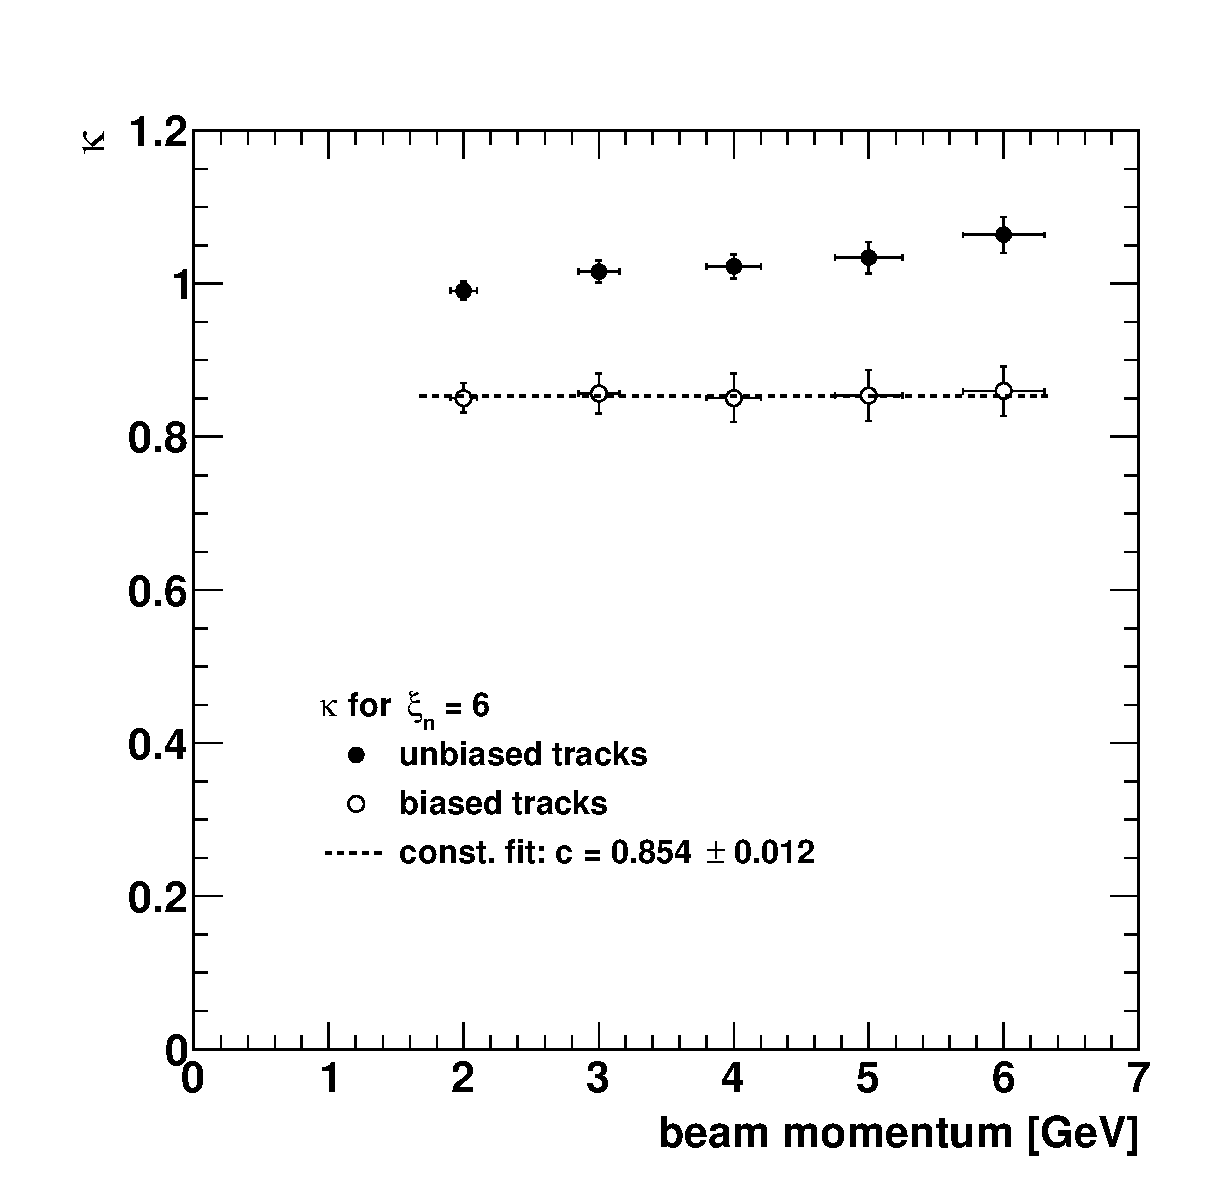
\includegraphics[width=0.49\textwidth]{figures/kappa}
  \caption[HL Factor]{
  The global factor $\kappa$ to equation~(\ref{eq:multiplescattering}) is plotted against beam energy.
  }
  \label{fig:HL_factor}
\end{figure}

Furthermore, the method has been repeated for various sensor thresholds.
The threshold applied to each telescope sensor is a critical parameter for the telescope performance.
A higher threshold reduces the amount of fired pixels which results in smaller and fewer clusters found on average on a plane and thus limiting the number of reconstructible tracks.
This reduces the telescope triplet efficiency, which is defined as the ratio of isolated, upstream triplets with a corresponding hit on plane\,3 within an acceptance range $d$
 around the triplet extrapolation to the overall number of isolated, upstream triplets.
A margin $d = 50\,\micro\meter$ is chosen for 6\,GeV and $\dz = 20\,\milli\meter$ and is additionally scaled with the inverse energy and the plane distance $\dz$ between measurements. 
In figure~\ref{fig:resivsenergy_thresh}~(A) the telescope triplet efficiency dependence on the sensor threshold is shown for various beam energies and sensor spacings.
Statistical uncertainties are negligible.
Systematic uncertainties are insignificant due to a precise alignment and the sufficiently large margin $d$.  
For thresholds $\noise = 5$ and $\noise = 6$ the efficiency is measured to $99.6\,\%$ and $99.4\,\%$.
With increasing threshold, the efficiency decreases to $82\,\%$ at $\noise = 12$. 
The efficiency varies by less than 0.1\,\% between different geometries and energy settings at thresholds $\noise = 5$ and $\noise = 6$. 

\begin{figure}[hb]
  \centering
  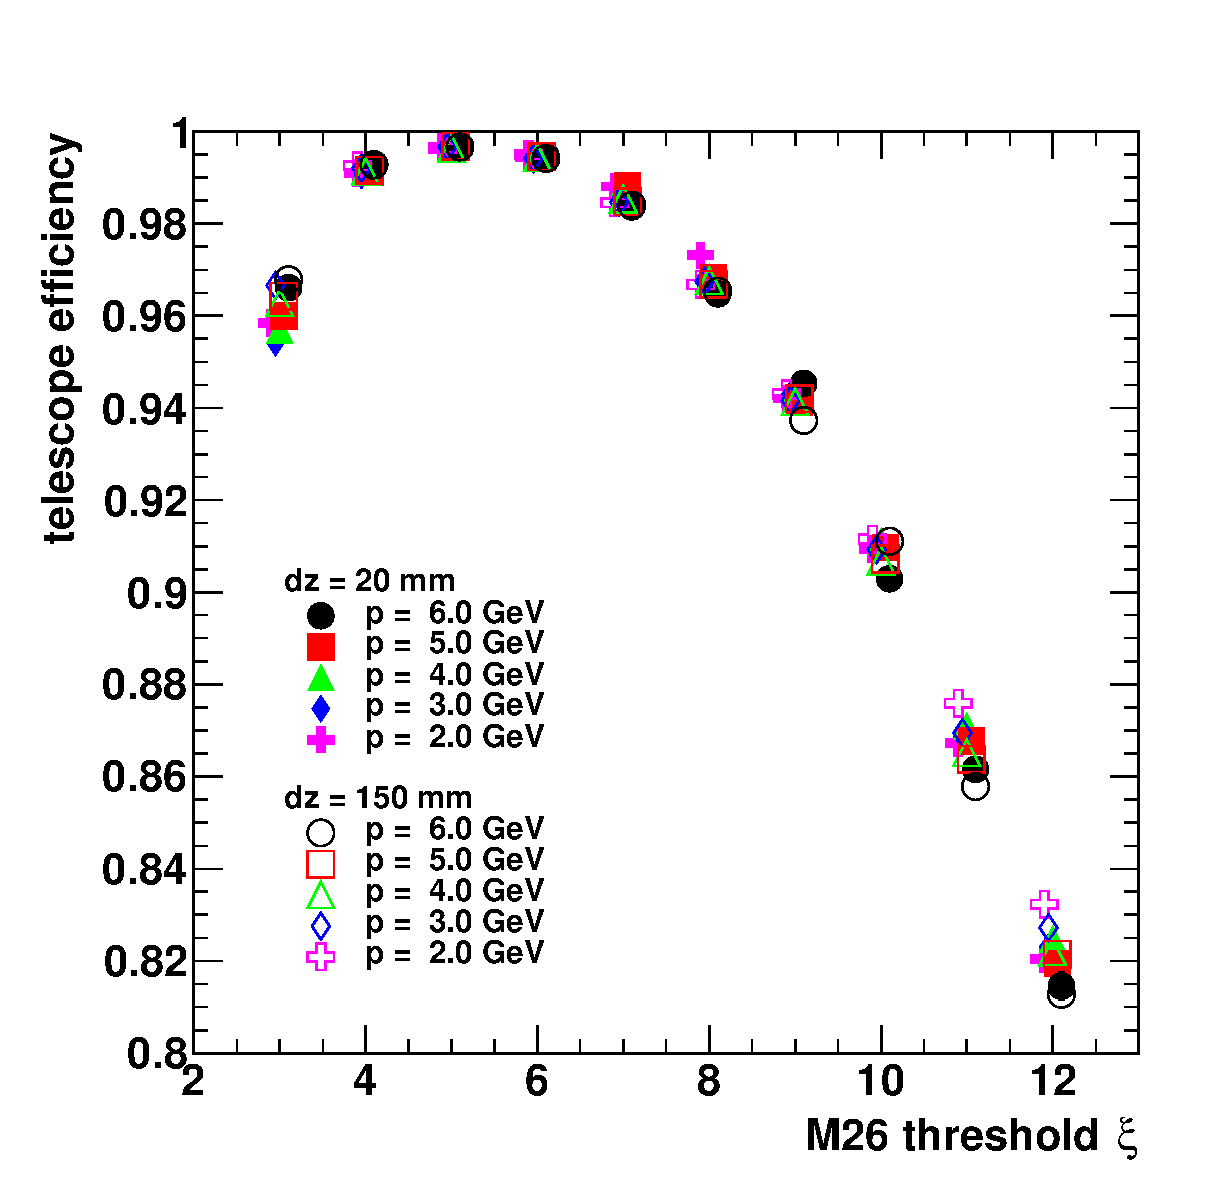
\includegraphics[width=0.49\textwidth]{figures/effi_vs_thres}	\put( -36,160){(A)}
  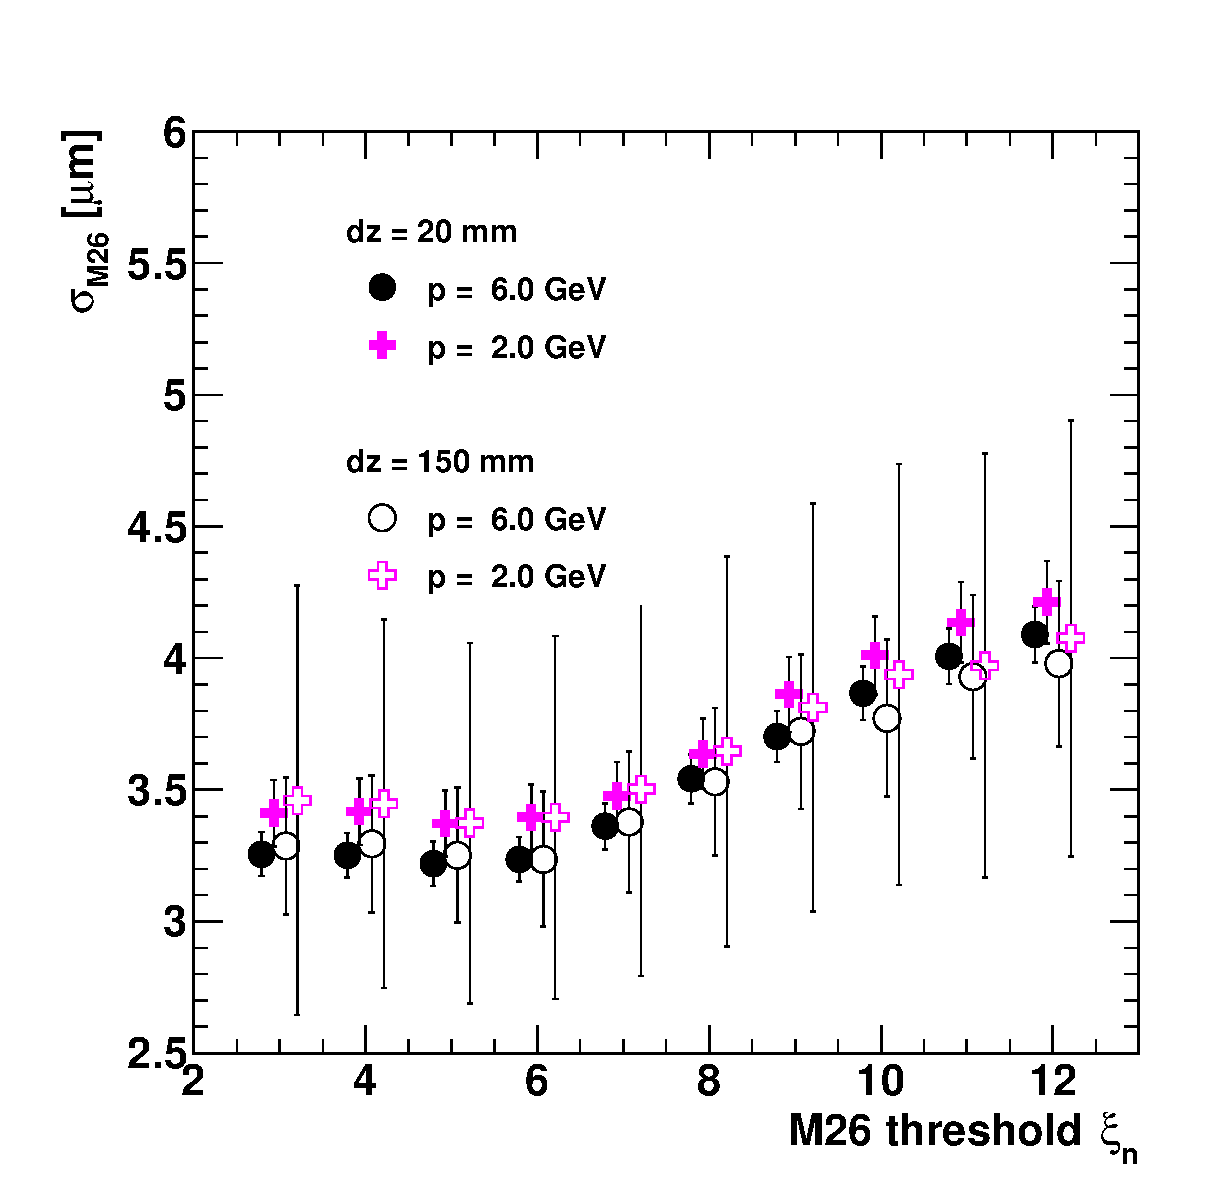
\includegraphics[width=0.49\textwidth]{figures/reso_vs_thres}	\put( -36,160){(B)} % was resi_thresh_errors
  \caption[Telescope intrinsic sensor resolution for different threshold settings, beam energies and geometries~\cite{ref:thomas}]{
(A) Average efficiency of all telescope sensors for different beam energies and sensor spacing vs.~applied threshold.
%An efficiency decline with increasing threshold can be observed.
(B) The measured intrinsic resolution of the $\sigma_{\textrm{M26}}$ for different beam energies $p$ and sensor spacing $\textrm{d}z$ as a function of the applied sensor threshold $\noise$.
In both images values are shifted on the $x$-axis for improved legibility.}
  \label{fig:resivsenergy_thresh}
\end{figure}

The threshold level affects not only the efficiency, but also the intrinsic resolution. 
With an increased threshold, a hit is formed on average from smaller clusters which deteriorates its position estimate. 
A deterioration also occurs towards lower thresholds, which allow for an increased number of noise induced signals to pass the zero-suppression on the chip.
%Figure~\ref{fig:effi} shows the efficiency distribution over a sensor plane.
%As maximum distance $100\,\micro\meter$ is considered.
%A noisy pixel column at $Y \approx -8\,\milli\meter$ can be observed.
%This column was masked during the converter step in the \texttt{datura-noDUT} example and subsequently is not used during the analysis. 
%\\{comment hj: datura-noDUT is jargon}
%Disregarding this area, an overall average efficiency over $98\,\%$ is observed.
%each resulting in an estimate for $\sigmai$ as a function of the set threshold $\noise$. 
Figure~\ref{fig:resivsenergy_thresh} (B) shows the intrinsic sensor resolutions $\sigmai$ derived from the measurements for different beam energies and plane distances as a function of the applied sensor threshold.
The minimum of $\sigmai$ is reached for a sensor threshold setting of $\noise = 5$.
The spread in intrinsic resolution for different energies is less than $0.1\,\upmu\meter$ for thresholds $\noise = 5$ and $\noise = 6$. 
A previous measurement and analysis~\cite{ref:j.behrmeasurements} taken at $\noise10$ yielded $\sigma_{\textrm{M26}} = (4.35\,\pm\,0.10)\,\micro\meter$,
 which seems to overestimates the intrinsic resolution. 



\subsection{Track resolution predictions using General Broken Lines}

%The track resolution of a beam telescope represents the accuracy with which a track can be pointed on a DUT. 
% In case multiple scattering cannot be neglected, it can be expressed as
% \begin{equation}
%  \sigmap^2 = \sigma_{\textrm{Tel}}^2 + \sigma_{\textrm{MS}}^2
% \end{equation}
% 
% \noindent
Using the measured intrinsic resolution, the known telescope plane material budget $\epsmimo = 7.6\cdot 10^{-4}$ and the material budget of a DUT $\epsdut$,
 predictions of the expected track resolution at the actual DUT position $\zdut$, c.f.\ figure~\ref{fig:datura_sketch}, can be made.
Therefore, it is possible to perform an a priori calculation of the optimal telescope geometry for a certain measurement set-up. 
In this section, $\zdut$ is assumed to be in the centre between plane\,2 and plane\,3.

%Track resolutions in this section refer to the achievable track resolution using a \textit{symmetric six M26 planes plus DUT} configuration. 
%This is referred to as \textit{user configuration}, also shown in figure~\ref{fig:datura_sketch}, while the set-up used in section~\ref{sec:measurements} is referred to as \textit{gauge configuration}. 

\begin{figure}[t]
  \centering
  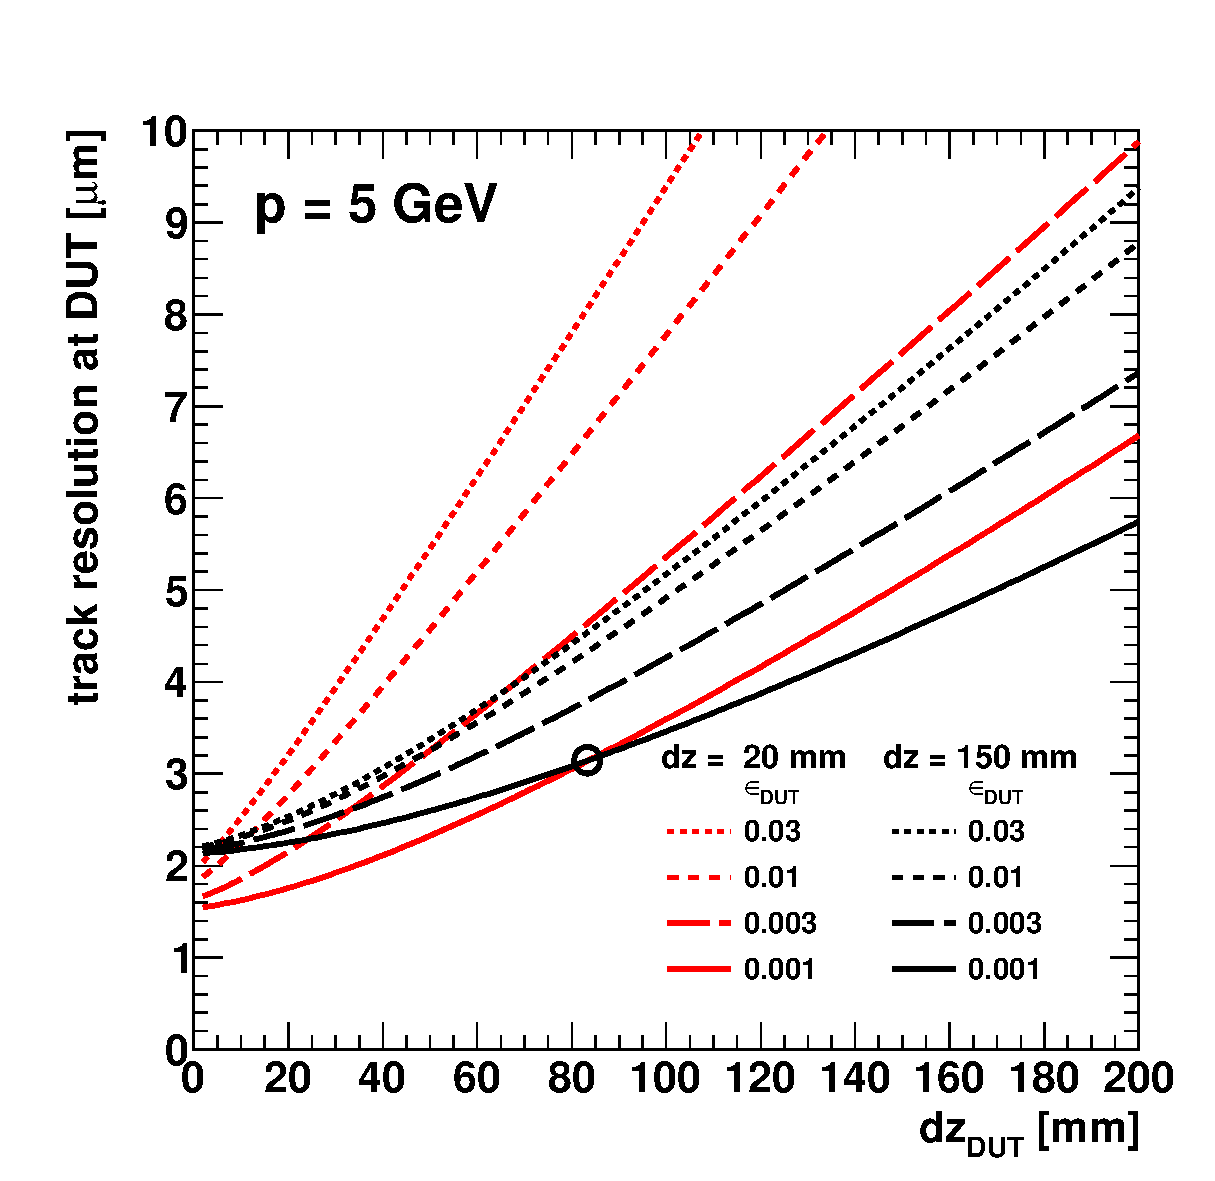
\includegraphics[width=0.49\textwidth]{figures/trackres_vs_dzdut_DESY}\put(-162,32){(A)}
  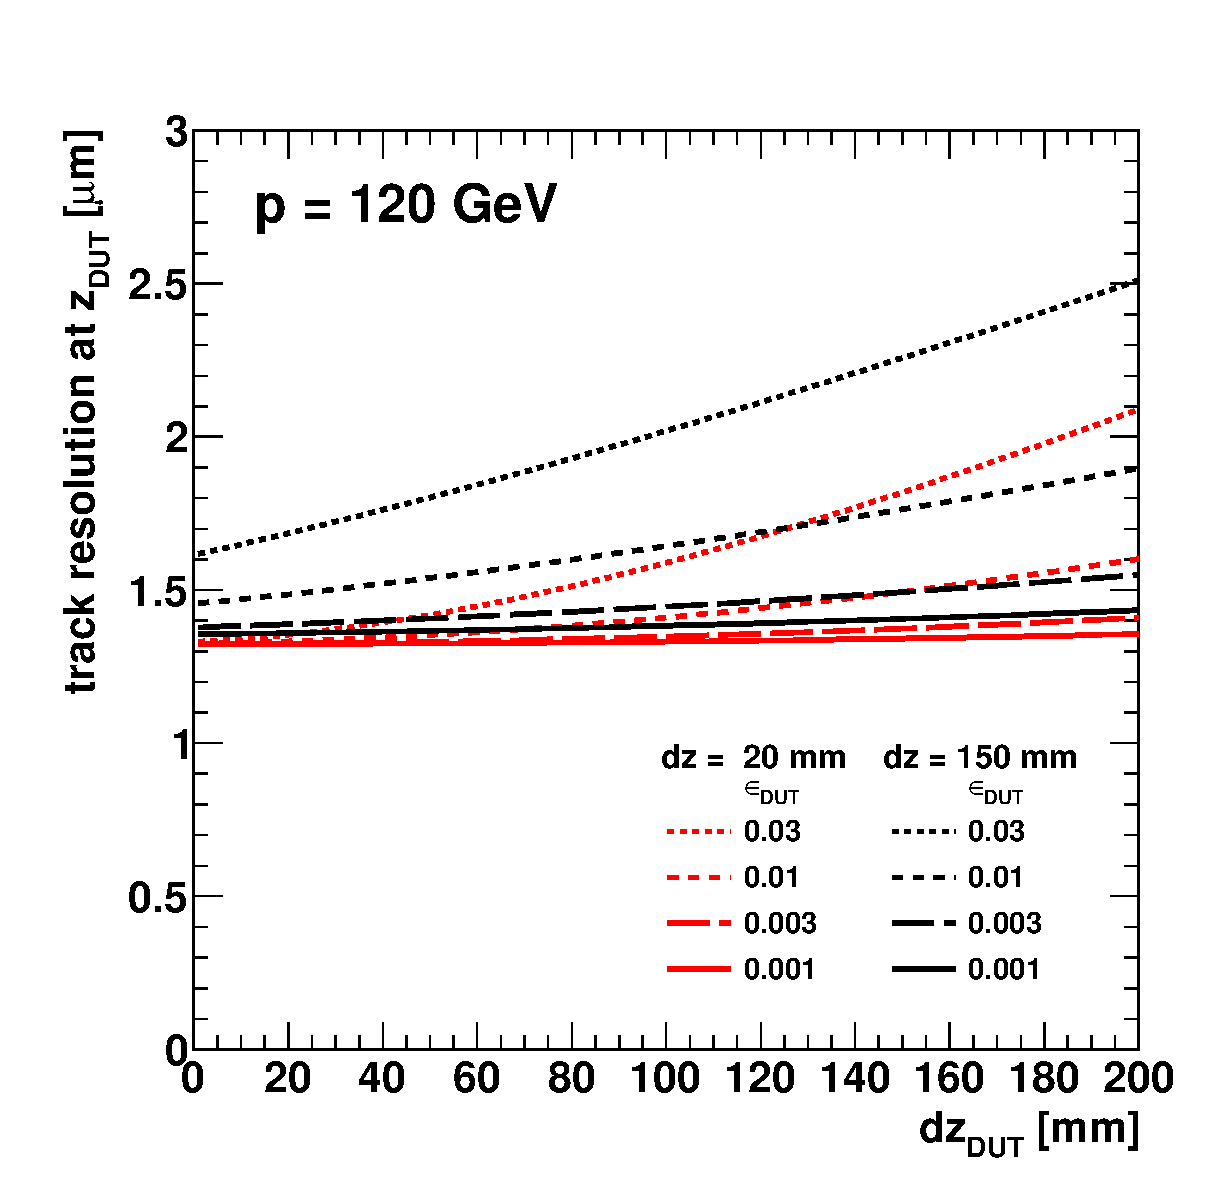
\includegraphics[width=0.49\textwidth]{figures/trackres_vs_dzdut_SPS} \put(-162,32){(B)}
  %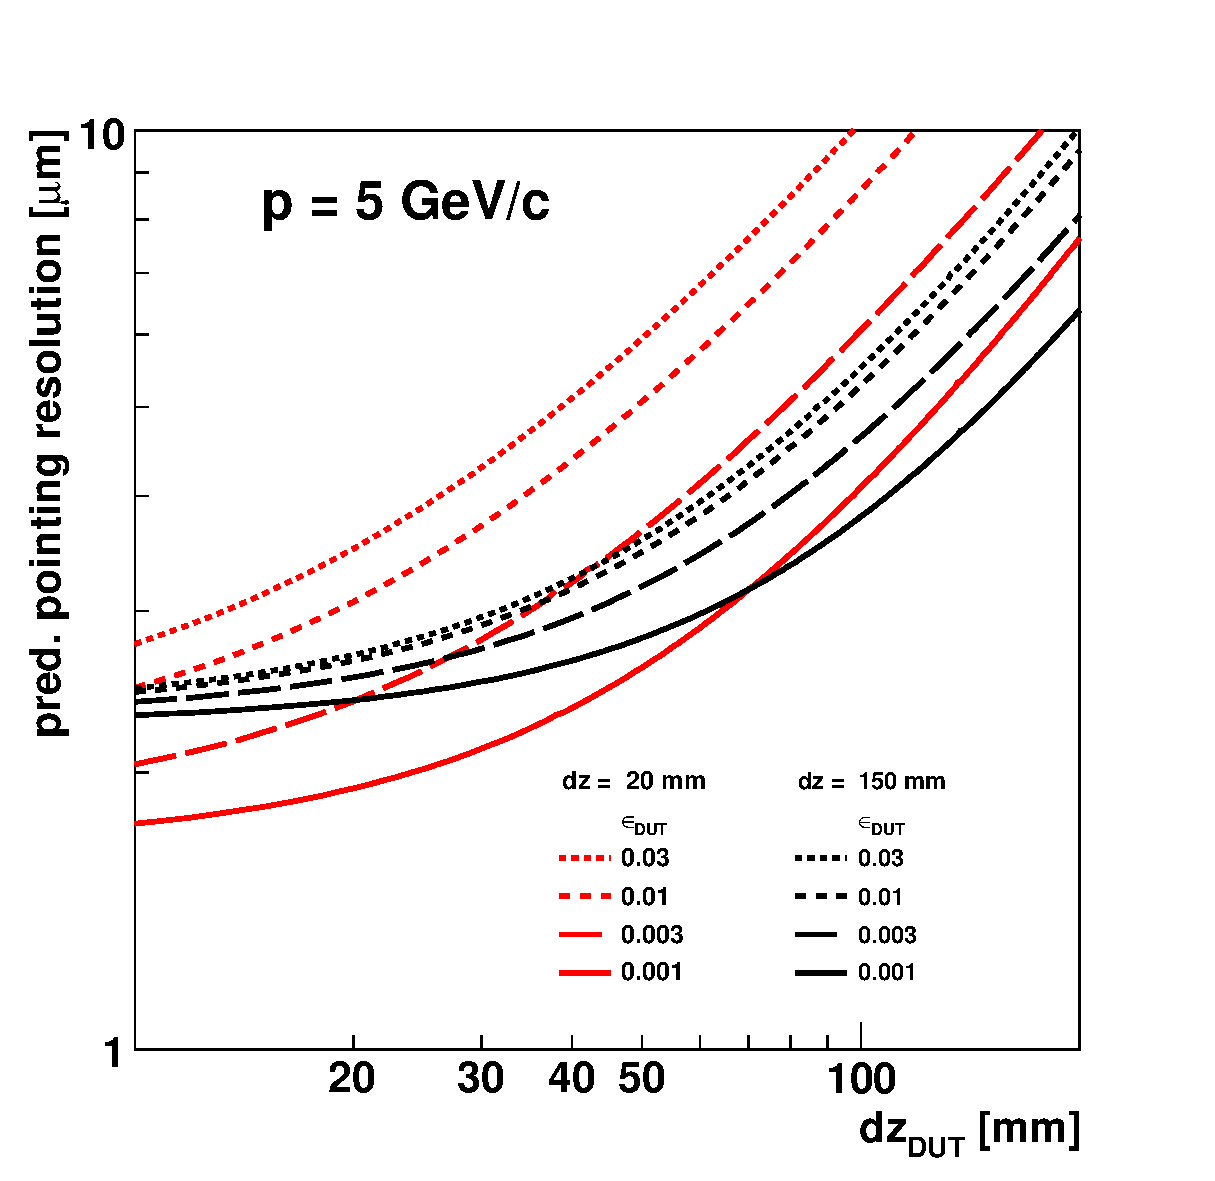
\includegraphics[width=0.49\textwidth]{figures/CalcResoVsDzdut_Desy_loglog_2}
  %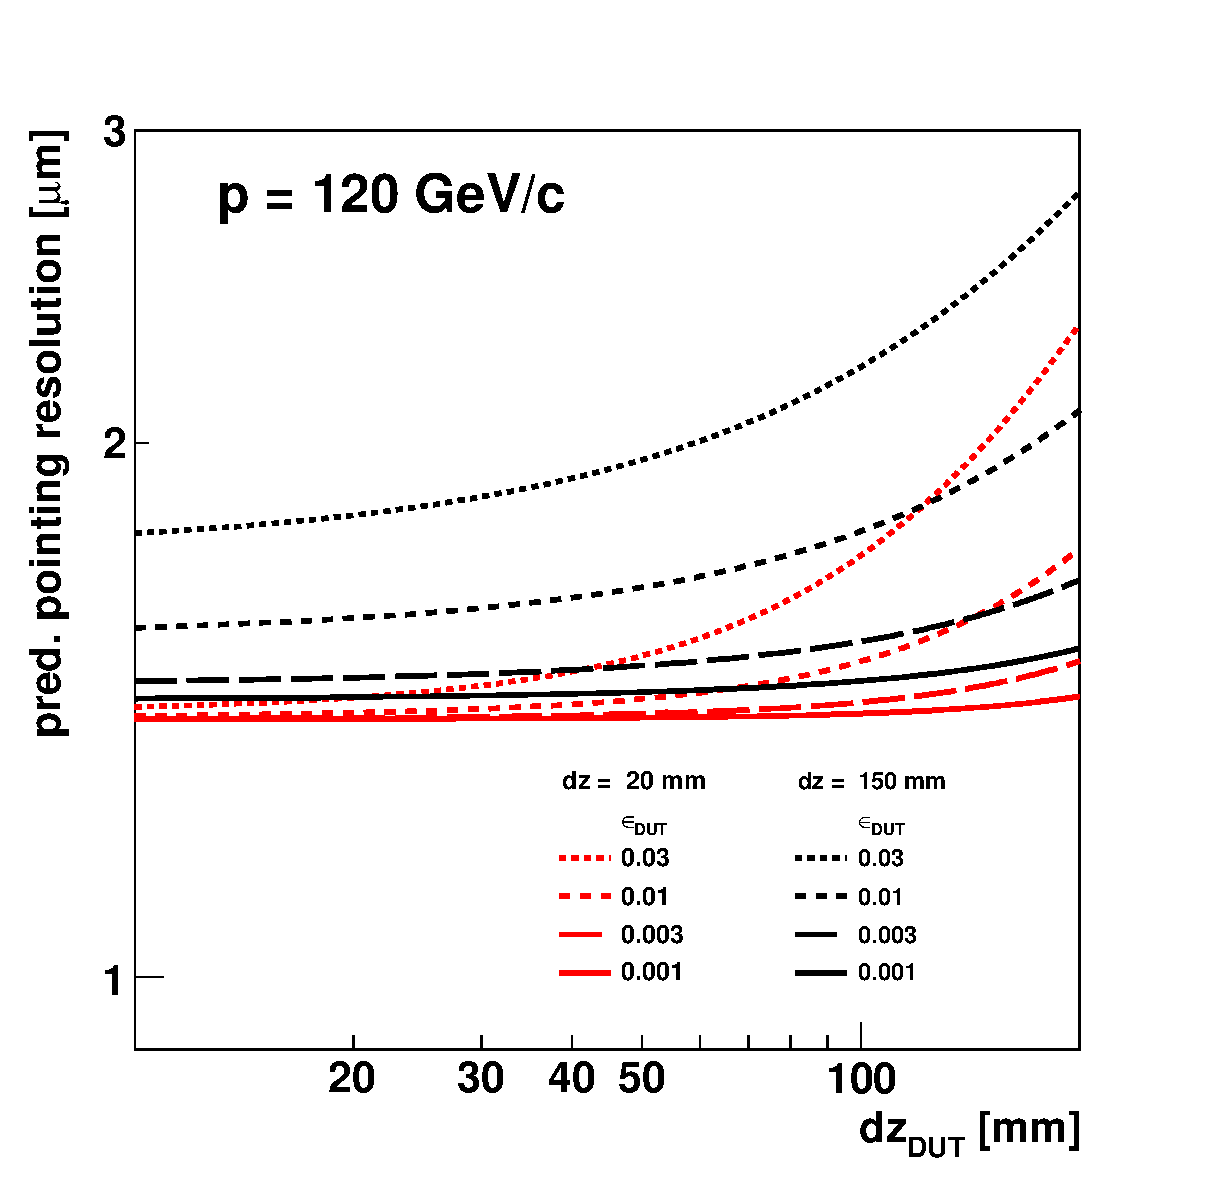
\includegraphics[width=0.49\textwidth]{figures/CalcResoVsDzdut_Cern_loglog_2}
  \caption[Track resolution for various material budgets as a function of the distance between DUT and neighbouring planes]{
  The track resolution for various material budgets is shown as a function of the equidistant spacing between DUT and neighbouring planes at 5\,GeV (A), and 120\,GeV (B)
  at the centre of the beam telescope ($\zdut$).}
  \label{fig:CalcResos_dzdut}
\end{figure}

Using the GBL formalism, the track resolution is analytically calculated at points of interest along the particle trajectory. 
The track resolution at the DUT for four different DUT material budgets $\epsdut$ is depicted as a function of the spacing $\dzdut$ in figure~\ref{fig:CalcResos_dzdut}.
Exemplified are two configurations with $\dz = 20\,\milli\meter$ and $\dz = 150\,\milli\meter$ at (A) DESY-II and (B) SPS beam energies. 
For $\dz = \dzdut = 20\,\milli\meter$ at 5\,GeV beam energy the track resolution at the DUT is 
\begin{equation}
 \sigmat(\zdut) = 1.75\,\pm\,0.02\upmu\meter
\end{equation}

\noindent
for $\epsdut = 0.001$.
%The uncertainty originates from an assumed uncertainties of 5\,\% on the beam energy and 10\,\% on the material budget. 
For SPS energies, a track resolution of $1.33\,\upmu\meter$ is predicted.
The shown resolutions monotonically increase with increasing $\dzdut$. 
In order to achieve the best possible resolution, the inner $\Mimosa$ planes should therefore be positioned as close as possible to the DUT, i.e.~$\dzdut$ is to be minimised. 
In addition, figure~\ref{fig:CalcResos_dzdut} shows, that the optimal plane spacing $\dz$ depends on the actual DUT size along the beam direction and its material budget.
For instance for a DUT with a material budget of $\epsdut = 0.001$ (solid lines) at 5\,GeV, a narrow configuration shows a higher track resolution for $\dzdut < 83\,\milli\meter$,
 while a wide configuration is best for $\dzdut > 83\,\milli\meter$.
The intersection is marked with a black circle in figure~\ref{fig:CalcResos_dzdut}. 
The position of the intersection depends on the material budget of the DUT $\epsdut$ and shifts to smaller $\dzdut$ with increasing material budget. 
%A DUT with a material budget of $\eps$
%In the wide (narrow) configuration, the predicted track resolution on the DUT is about $2.4\,\upmu\meter$ ($1.9\,\upmu\meter$) at $\dzdut = 20\,\milli\meter$ for DUTs with $\epsdut = 0.001$.
At SPS energies, the resolution functions for the wide and the narrow configuration do not intersect, with the narrow configuration showing a slightly better track resolution at the DUT. 
However, the difference is less than $0.5\,\micro\meter$ for $\zdut = 100\,\milli\meter$ even at $\epsdut = 0.03$. 



% Using the \textit{gauge configuration}, a comparison between the GBL calculations and the measurements can be performed.
% For this, the measured resolution has to be converted to the track resolution $\sigmap$ by correcting for the intrinsic resolution of the DUT $\sigmadut = \sigmam$
% 
% \begin{equation}
%  \sigmap = \sqrt{\sigmameas^2 - \sigmadut^2}.
%  \label{eq:sigmap}
% \end{equation}
% 
% \noindent
% This is shown in figure~\ref{fig:CalcResoP_DUT} (A) as a function of the beam energy. 
% The solid lines represent GBL calculations, while the triangles show the derived $\sigmap$ obtained from equation~(\ref{eq:sigmap}). 
% The hatched bands represent the calculated track resolution assuming $\sigmam = 3.43\,\upmu\meter$ with a standard deviation of $0.10\,\upmu\meter$ for the wide and the narrow configuration. 
% An excellent agreement between GBL calculations and the measurements is found. 
% For the limit towards high energies, or negligible multiple scattering, a track resolution of $1.6\,\upmu\meter$ is predicted. 
% The measurement at 120\,GeV confirms the prediction, 

In figure~\ref{fig:CalcResoP_DUT} the achievable track resolution at $\zdut$ as a function of the material budget is shown for a beam energy of 5\,GeV.
%Again, a minimal $\dzdut$ allows for the best possible resolution. 
Dashed and solid lines represent calculations for $\dz = 20\,\milli\meter$ and $\dz = 150\,\milli\meter$, respectively. 
The track resolution deteriorates with increasing $\epsdut$. 
The optimal plane spacing $\dz$ depends on the actual size requirements for the DUT along the beam direction and its material budget.
For instance, for a DUT with a material budget of $\epsdut = 0.002$, a plane spacing of $\dz = 20\,\milli\meter$ should be used, if $\dzdut$ is as small as 20\,mm. 
However, a plane spacing of $\dz = 150\,\milli\meter$ is preferred, if $\dzdut$ is 60\,mm or larger. 
Intersections are marked with open circles. 
For $\epsdut$ below (above) the intersection, a narrow (wide) configuration is preferable. 
The position of the intersection shifts to smaller material budgets with increasing $\dzdut$. 

\begin{figure}[tbp]
  \centering
  %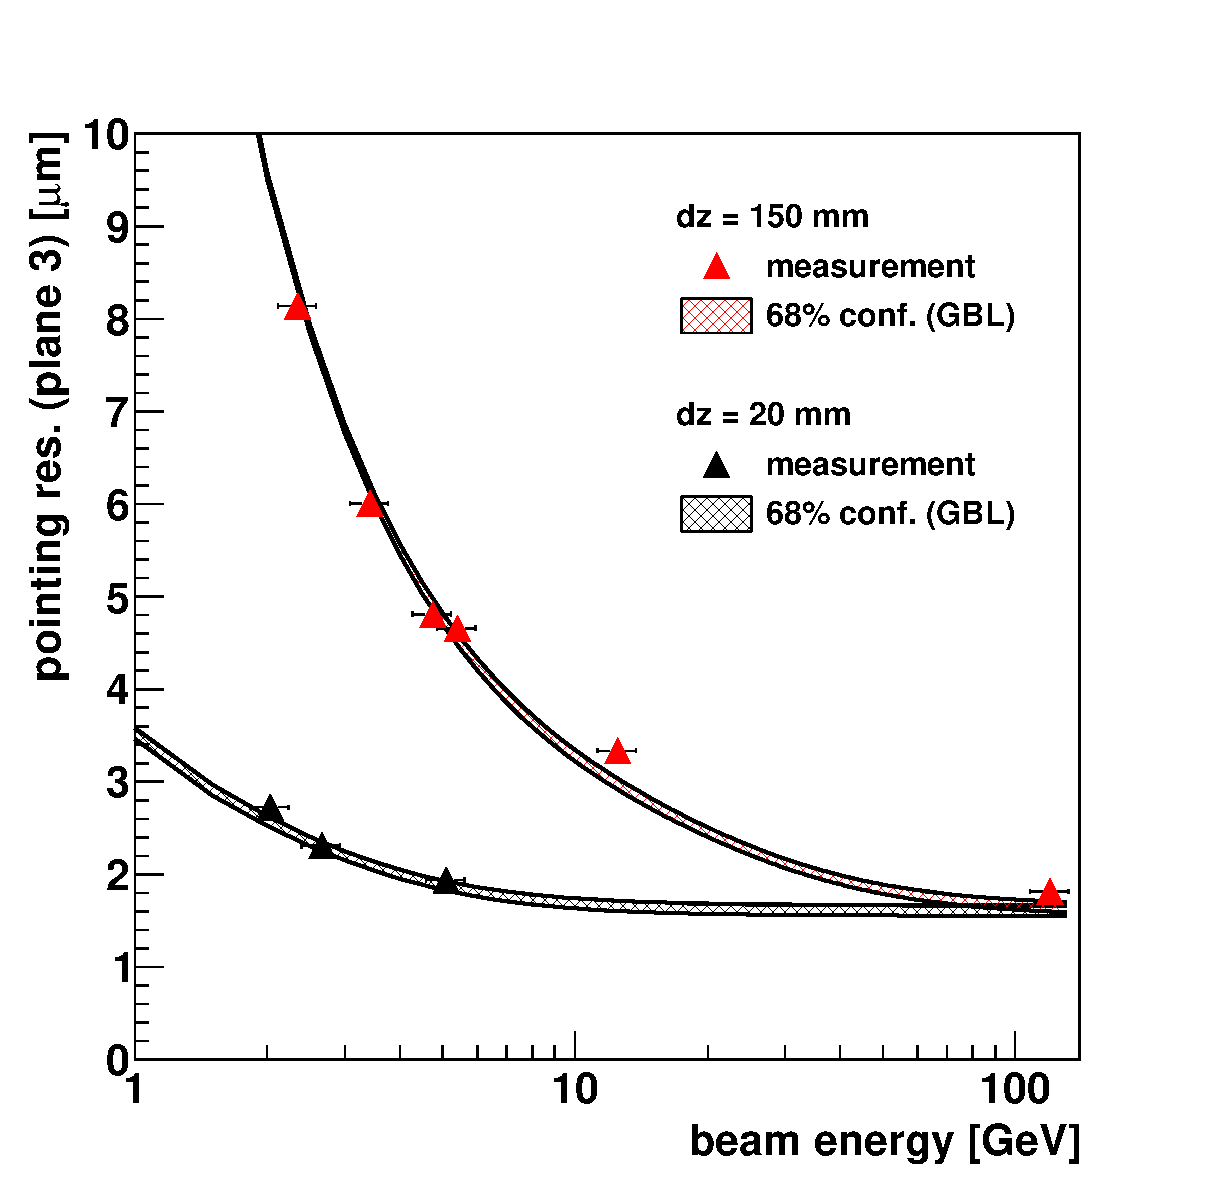
\includegraphics[width=0.49\textwidth]{figures/energy_plot}     \put(-175,40){(A)} % was CalcResoVsP
  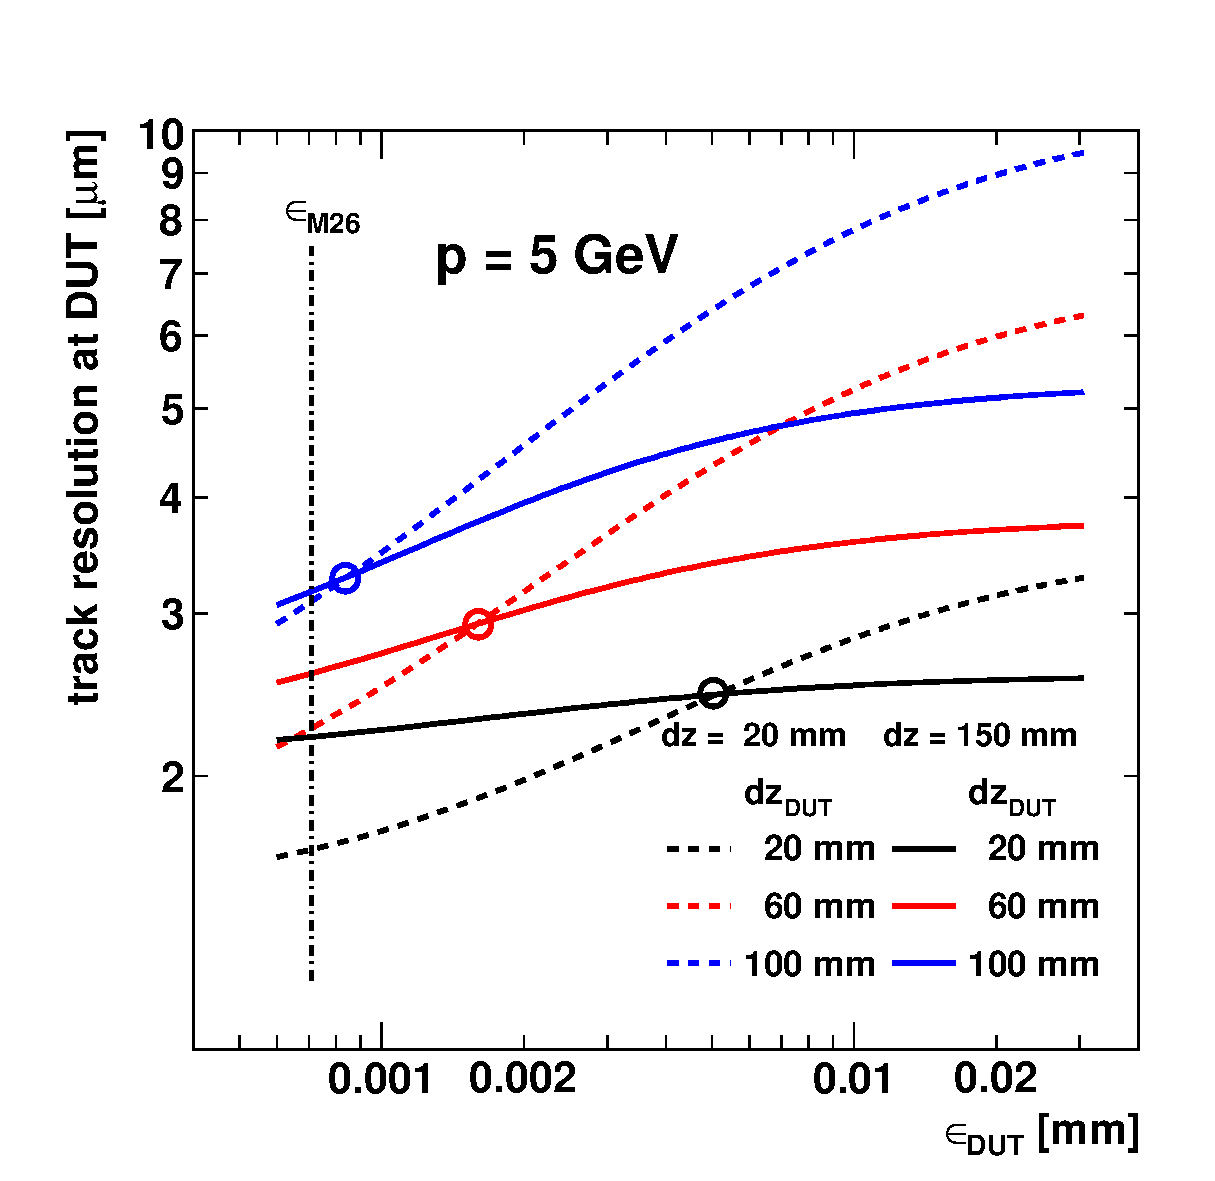
\includegraphics[width=0.49\textwidth]{figures/trackres_vs_epsdut_DESY} %\put(-155,40){(B)}
%               \put(-175,107.5){$\bigcirc$}
%  \color{blue} \put(-161,102.5){$\bigcirc$}
%  \color{green}\put(-143,96.5){$\bigcirc$}
%  \color{red}  \put(-113,90){$\bigcirc$}
%  \color{black}
   \caption[Track resolution as a function of the beam energy]{
   %(A) The measured (triangles) and calculated (lines) track resolution at plane $3$
   % for the wide (red) and the narrow (black) set-up is shown as a function of the beam energy for the \textit{gauge configuration}~\cite{ref:thomas}. 
   %The solid lines form bands representing the standard deviation of $0.10\,\upmu\meter$ of the intrinsic resolution.
   %The theoretical limit of about $1.6\,\upmu\meter$ for plane\,3 is indicated as a dashed line.
   %Track resolutions derived from the measured resolutions at plane 3 for various energies and plane spacings are shown as crosses.
   The calculated track resolutions at the DUT for two geometries are shown as a function of $\epsdut$ at $\zdut$ at a beam energy of 5\,GeV. 
   Note the double logarithmic scales. 
   }
 \label{fig:CalcResoP_DUT}
\end{figure}

A web tool yielding compatible results in comparison with the GBL calculations is available~\cite{webtool}. 
The tool calculates track resolutions for a fixed set-up with six planes and one DUT in the centre. 
A more versatile GBL track resolution calculator allowing for all possible geometries is also available~\cite{gbltool}. 
